% Класс документа пока не окончательный, сильно сомневаюсь, что article лучший
\documentclass[a4paper,12pt]{extarticle} 
% Подключаем шрифты,кодировки,русские переносы
\usepackage{cmap}
% подключается пакет, позволяющий улучшить вид пдф документа(как я понял)
\usepackage[utf8x]{inputenc}
% подключаем кодировку шрифтов для вносимых файлов
\usepackage[T2A]{fontenc}
\usepackage[russian,english]{babel}
% подключаем перенос и распознование слов, русский в приоритете
\usepackage{indentfirst}
% Отступ в начале абзаца
\usepackage{
	amssymb,
	amsfonts,
	amsmath,
}
% Пакеты американского математ. сообщества, красивый вид формул и текста внутри
\usepackage{
	wrapfig,
	graphicx,
	caption,
	subcaption,
	tikz,
}
% Обтекаемые объекты, рисунки, подписи и прочее
\usepackage{
	pgfplotstable,
	pgfplots,
	booktabs,
	colortbl,
	array
}
\pgfplotsset{compat=newest}
% таблицы, графики
\usepackage{geometry}
\usepackage{fancyhdr}
% границы, контитулы, и прочее


\geometry
	{
	left=2.2cm,
	right=2.2cm,
	bottom=2cm,
	top=2cm,
	}
% границы документа

\usepackage{setspace}
% убирает гигантские размеры оглавления
\linespread{1.3}
% междустрочный интервал

\pagestyle{fancy}
\fancyhead{}
% пустая шапка контитула
\fancyhead[R]{\authors}
% На правой стороне страницы авторы и науч.рук.
% \fancyhead[L]{\shortlabname}
 % Слева название лабы
\fancyfoot{}
\fancyfoot[C]{\thepage}
% номер страницы снизу по середине
\renewcommand{\contentsname}{Оглавление}
% переводим на русский язык оглавление
\usepackage{secdot}
\sectiondot{subsection}
% Ставит злосчастные точки в главах, ибо не по госту
% Преамбула почти слизана у Федора Сарафанова https://github.com/FedorSarafanov/RLC/blob/master/text/diss.tex

\usepackage{xcolor}
\usepackage{float}
\usepackage{hyperref}
% \hypersetup{unicode=true}
% \definecolor{linkcolor}{HTML}{799B03} % цвет ссылок
% \definecolor{urlcolor}{HTML}{799B03} % цвет гиперссылок

% \hypersetup{pdfstartview=FitH,  linkcolor=linkcolor,urlcolor=urlcolor, colorlinks=true}
\begin{document}
\sloppy
\def\authors{Есюнин М.В., Есюнин Д.В.}
\def\sciadviser{Пикулин В.Д.}
\def\labname{Опыт Франка-Герца}
\renewcommand{\contentsname}{Оглавление}
\renewcommand{\figurename}{Рис.}
\renewcommand{\vec}{\mathbf}
\renewcommand{\phi}{\varphi}
\renewcommand{\kappa}{\varkappa}
% нормальный вид вектора, фи и каппа
\renewcommand{\Re}{\operatorname{Re}}
\renewcommand{\Im}{\operatorname{Im}}
% меняем номрмальное начертание Re and Im

\begin{titlepage}

\begin{center}

	\textsc{Нижегородский государственный университет имени Н.\,И. Лобачевского}
	\vskip 4pt \hrule \vskip 8pt
	\textsc{Радиофизический факультет}

	\vfill

	{\Large\labname}

\end{center}

\vfill

\begin{flushright}
	{Работу выполнили студенты\\ \authors\\ 430 группы\\ \vskip 14pt преподаватель:\\ \sciadviser}
\end{flushright}

\vfill

\begin{center}
	Нижний Новгород, \the\year
\end{center}

\end{titlepage}
\begin{spacing}{1.2}
	\tableofcontents
\end{spacing}
\newpage
\section{Теоритеческое введение}
На основании проведенных экспериментов Резерфордом в 1911 г. была построена планетарная модель атома. Но устойчивость такого атома и характер его спектров невозможно было объяснить с точки зрения известных тогда классической механики и электродинамики. Для устранения указанного противоречия Н. Бор в 1913 г. предложил квантовую теорию строения атома, в основе которой лежат следующие постулаты.
\begin{enumerate}
\item {Атомы могут длительно пребывать только в определенных энергетических состояниях. В этих состояниях они обладают энергиями $E_0,E_1,E_2,\ldots,E_n,$ образующими дискретный ряд. При движении электронов по соответствующим этим состояниям стационарным орбитам никакого излучения или поглощения энергии не происходит. Всякое изменение энергии атома может происходить только скачком в результате перехода между указанными выше энергетическими состояниями.
}
\item {При переходе из одного энергетического состояния $E_m$ в другое $E_n$ поглощается или излучается строго определенная порция (квант) электромагнитной энергии. Энергия кванта связана с частотой излучения $\nu$ следующим отношением:
\begin{equation*}
	h\nu = E_m-E_n
\end{equation*}
где $h$ - постоянная Планка.
}
\end{enumerate}

Ставшие классическими эксперименты, выполненные в 1913 г. Д.Франком и Г.Герцем, непосредственно подтвердили справедливость квантовых постулатов Бора. В опыте Франка-Герца исследуются процессы столкновения электронов с атомами газа. Упрощенная схема экспериментальной установки приведена на рис. В баллоне лампы \textit{Л} заполненной исследуемым газом, находятся три электрода: раскаленный катод \textit{К}, являющийся источником электронов, сетка \textit{С} и анод \textit{А}. Между сеткой и катодом прикладывается разность потенциалов $\phi_y=\phi_c-\phi_k$, ускоряющая
электроны (потенциал сетки по отношению к катоду $\phi_y$ называют ускоряющим потенциалом). Разность потенциалов между анодом и сеткой имеет, как правило, противоположный знак и носит название потенциала задержки $\phi_\text{з}=\phi_a-\phi_c<0$.

В ходе выполнения эксперимента снимается анодно-сеточная характеристика газонаполненной лампы, т.е. зависимость анодного тока $i_a$ от ускоряющего потенциала $\phi_y$ при постоянном потенциале задержки $\phi_\text{з}$. Типичный вид этой характеристики приведен на рис. \ref{}. На начальном участке характеристики по мере увеличения $\phi_y$ наблюдается монотонный рост анодного тока. В этом режиме вылетающие из катода электроны при движении к сетке приобретают сравнительно малую энергию $W_e$ и сталкиваются с атомами газа упруго. При таких столкновениях кинетическая энергия атома изменяется слабо - на величину порядка

\begin{equation*}
	\Delta W \thicksim W_e \frac{m}{M} \ll W_e
\end{equation*}

где $m$ и $M$ - массы электрона и атома соответственно, а внутреннее состояние атома не меняется. Поскольку при столкновениях атомы отбирают у электронов лишь незначительную часть энергии, последние, проходя через некоторую эквипотенциальную поверхность с потенциалом $\phi$, имеют энергию, примерно равную $e\phi$ (здесь не учтена начальная скорость вылета электронов с катода).
При $\phi_y>\phi_\text{з}$ электроны пролетают через сетку, имея
энергию, достаточную для преодоления задерживающего потенциала, и достигают анода. Как и в обычных электронных лампах, с ростом потенциала сетки $\phi_y$ анодный ток возрастает. Этот процесс продолжается до тех пор, пока $\phi_y$ не достигнет величины так называемого первого критического потенциала $\phi_1$ (его называют также резонансным потенциалом), при котором электроны приобретают энергию, достаточную для возбуждения атома. Столкновения электронов, имеющих энергию $e\phi_1$, с атомами могут происходить неупруго. При этом электрон в процессе столкновения всю свою энергию передает атому. Величина критического потенциала $\phi_1$ связана с разностью энергии возбужденного $E_1$ и невозбужденного $E_0$ атомов законом сохранения энергии:

\begin{equation*}
	e \phi_1=E_1-E_0
\end{equation*}

Электроны, потерявшие энергию при неупругих столкновениях, не могут преодолеть задерживающего поля между анодом и сеткой и "вылавливаются" последней, поэтому анодный ток с дальнейшим ростом $\phi_y$ уменьшается. Так возникает падающий участок на анодно-сеточной характеристике.
При дальнейшем увеличении $\phi_y$ поверхность с потенциалом $\phi_1$ (а, следовательно, и область неупругих соударений) смещается от сетки к катоду. При $\phi_y \geq \phi_1+|\phi_y|$ электроны, испытавшие неупругие соударения на пути к сетке, вновь могут набрать энергию, превышающую $e\phi_1$, и анодный ток опять возрастает с ростом $\phi_y$. Начиная со значения $\phi_y \geq 2\phi_1$, электроны на своем пути могут дважды неупруго столкнуться с атомами и, потеряв энергию после второго столкновения, не преодолеть задерживающий потенциал. Это приведет к появлению второго провала на анодно-сеточной характеристике. Аналогичным образом происходит падение тока и при более высоких потенциалах $\phi_n=n\phi_1$.

Таким образом, опыт Франка-Герца убедительно подтверждает справедливость первого постулата Бора: атом действительно поглощает энергию только определенными дискретными порциями.

Франк и Герц, выполнив свои эксперименты с парами ртути, показали, что минимальная энергия, которую способен поглотить атом ртути, составляет $4.9$ эВ, т.е. величина резонансного потенциала равна $4.9$ В. Они установили также, что возбужденные до резонансного уровня атомы ртути, переходя в невозбужденное состояние, являются источником ультрафиолетового излучения с длиной волны 2537 \AA. Этот результат находится в полном соответствии со вторым постулатом Бора.

\section{Экспериментальная часть}

В экспериментальной установке используется переделанная манометрическая лампа типа ЛМ-2: ее V-образный катод заменен прямой нитью накала, в результате вся система электродов приобрела цилиндрическую симметрию. Силовые линии электрического поля внутри лампы имеют весьма сложную форму. Это обусловлено несколькими причинами: во-первых, конструктивными особенностями сетки (шаг ее витков соизмерим с расстояниями от сетки до катода и анода); во-вторых, наличием отрицательного пространственного заряда у катода (как в обычной электронной лампе) и, наконец, неэквипотенциальностью самой поверхности катода, к концам которого приложено накальное напряжение. В таких условиях, даже экспериментально подобрав оптимальное давление заполняющего лампу газа, на анодно-сеточной характеристике удается получить лишь два хорошо выраженных максимума тока. Но для определения резонансного потенциала этого вполне достаточно.

Рассмотрим качественно процессы, происходящие в лампе. Подлетая к эквипотенциальной поверхности $S_1$, с критическим потенциалом $\phi_1$, электроны имеют энергию, достаточную для возбуждения атома. Однако неупругие столкновения происходят вблизи $S_1$ случайно в пределах длины свободного пробега электронов $\lambda$, т. е. существует область неупругих столкновений $\Omega$ - слой, примыкающий к поверхности $S_1$, (в сторону нарастания потенциала) толщиной порядка $\lambda$. Очевидно, что с ростом величины ($\phi_y$ этот слой вначале появляется у витков сетки.

Энергии электронов, испытывающих соударения в различных точках слоя, могут различаться на величину порядка

\begin{equation*}
	\Delta W_{\lambda} = e \lambda \frac{d\phi}{dn}
\end{equation*}
где $\displaystyle\frac{d\phi}{dn}$ - производная потенциала по нормали к $S_1$.

Разброс по энергиям на $\Delta W_\lambda$ расширяет максимум анодно-сеточной характеристики и уменьшает крутизну падающего участка.

Проще всего это понять на "плоской модели" со сплошной сеткой, проницаемой для электронов. В такой модели электрические поля между катодом и сеткой, сеткой и анодом однородны, а эквипотенциальные поверхности, показанные на рис. \ref{} штриховыми линиями, представляют собой плоскости, параллельные электродам.

Анодный ток будет тем меньше, чем больше неупругих соударений происходит в объеме $\Omega$. В этой модели минимум анодного тока будет наблюдаться тогда, когда поверхность $S_1$ с потенциалом $\phi_1$ сместится от сетки к катоду на длину $\lambda$, т.е. при ускоряющем потенциале на сетке

\begin{equation*}
	\phi_{min}=\phi_1+\lambda\frac{d\phi}{dn}
\end{equation*}

Уменьшение величины $\displaystyle\lambda\frac{d\phi}{dn}$, очевидно, сужает максимум анодно-сеточной характеристики (см. рис. \ref{}). Одновременно увеличивается крутизна ее падающего участка.

Аналогичная картина будет иметь место и в реальной лампе. Таким образом, экспериментальная погрешность определения критического потенциала оценивается как:
\begin{equation*}
	\Delta \phi \thicksim \lambda \frac{d\phi}{dn}
\end{equation*}

Заметим далее, что если на длине свободного пробега электрон может набрать энергию, большую разности энергий двух уровней $E_n-E_1$, то возможно возбуждение всех уровней с энергией, меньшей $E_n$, и даже ионизация атома, если $E_n-E_1$, больше энергии ионизации. Поэтому уменьшение длины свободного пробега $\lambda$ (за счет увеличения давления газа внутри лампы) позволяет не только увеличить точность определения резонансного потенциала, но и избежать перекрытия различных ступеней возбуждения. С другой стороны, слишком сильное уменьшение $\lambda$ нецелесообразно, т.к. при этом электроны до прихода в область неупругих соударений $\Omega$ испытывают много упругих столкновений, что увеличивает их разброс по энергиям, и, следовательно, уменьшает точность определения резонансного потенциала.

Для того чтобы качественно объяснить ход анодно-сеточной характеристики, необходимо рассмотреть, как изменяется поверхность $S_1$ (а с ней и область $\Omega$) с ростом $\phi_y$. На рис. \ref{} изображены сечения эквипотенциальных поверхностей плоскостью, проходящей через ось симметрии лампы, для последовательно увеличивающихся значений отношения $\displaystyle\phi_\text{з}/\phi_y$ {справа на этих рисунках показано примерное распределение потенциалов в лампе). Сплошной линией на этих рисунках показана эквипотенциальная поверхность $S_a$, имеющая потенциал $\phi_a$ (относительно катода).

Потенциальный рельеф, изображающий энергию электрона в различных точках рассматриваемого сечения, можно образно представить в виде полотна, натянутого наклонно со спуском к аноду; у проволоки сетки полотно оттянуто вниз. На пути от катода к аноду, проходящему посредине между витками сетки, рельеф или непрерывно понижается (рис. \ref{} и \ref{}), или же на этом пути имеется впадина (рис. \ref{}).

Будем увеличивать $\phi_y$ при постоянном $\phi_\text{з}$, как это необходимо для снятия анодно-сеточной характеристики. Когда $\phi_y$ достигнет значения $\phi_1$, у витков сетки появится область неупругих соударений $\Omega$, которая при дальнейшем увеличении $\phi_y$ удаляется от витков сетки вслед за $S_1$. На рис. \ref{} показано приближенное расположение областей $\Omega$ для трех значений $\phi_y$, отмеченных на рис. \ref{}, как $\phi_1, \phi_{min}$, и $\phi'$ (области, отмеченные соответственно буквами а, б, в на каждом из рис. \ref{}). Хотя поверхность $S_a$ смещается при изменении $\phi_y$, на рисунках это не отражено, так как полагается, что , $\phi_1, \phi_{min}$, и $\phi'$ мало отличаются друг от друга.

С ростом $\phi_y$ от $\phi_1$ до $\phi_{min}$ область $\Omega$ растет вначале за счет увеличения толщины слоя (пока расстояние or $S_1$ до сетки меньше $\lambda$ ), а затем за счет увеличения площади поверхности $S_1$. Пропорционально растет число неупругих соударений и падает анодный ток. При $\phi_y=\phi_1+|\phi_\text{з}| \approx \phi_{min}$ поверхности $S_1$ и $S_a$ совпадут. Дальнейшее увеличение потенциала $\phi_y$ сопровождается выходом области $\Omega$ за поверхность $S_a$ в ту часть поля, где энергия электронов выше, чем на аноде (области "в" на рис. \ref{}). Электроны, столкнувшиеся здесь неупруго, как правило, попадают на анод, и анодный ток с ростом $\phi_y$ вновь начинает возрастать. (На сетку в этом случае летят лишь те электроны, которые потеряли энергию, находясь вблизи от дна воронки потенциального рельефа. При $\phi_\text{з}/ \phi_y \ll 1$ воронки неглубокие и таких электронов мало.)

На рис. \ref{} и \ref{} между частями $S_a$, огибающими соседние витки видны промежутки тем большие, чем меньше отношение $\phi_\text{з}/ \phi_y$. В этих промежутках потенциальный рельеф монотонно спадает на пути от катода к аноду, т.е. часть электронов попадает на анод, минуя область $\Omega$. Этим потоком электронов определяется минимальное значение тока при $\phi_y=\phi_{min}$. Для больших потенциалов задержки, когда реализуются структуры поля, изображенные на рис. \ref{}, электроны при $\phi_y=\phi_1+|\phi_\text{з}| \approx \phi_{min}$ могут попасть на анод только через область $\Omega$, поэтому ток в минимуме может доходить до нуля.

Совершенно аналогично объясняется наличие второго спадающего участка на анодно-сеточной характеристике при $\phi_y \geq 2\phi_1$.

Для некоторых газов, у которых величина резонансного потенциала не сильно отличается от потенциала ионизации, можно, используя эту же лампу, только при относительно больших потенциалах задержки ($\phi_\text{з}/ \phi_y \thicksim 1$), измерить также и потенциал ионизации.

Для этого можно использовать то обстоятельство, что при $|\phi_\text{з}|> \phi_y$, электроны, эмитированные катодом, не достигают анода, и анодный ток может быть вызван только положительными носителями заряда. В случае $|\phi_\text{з}|> \phi_y \geq \phi_i$ наличие анодного тока связано с процессами ионизации электронным ударом в окрестностях сетки. Когда $\phi_y$ достигнет значения $\phi_i$, у витков сетки появится область неупругих соударений, в которой энергия электронов будет достаточна для ионизации атомов газа, и возникнет ионный ток между сеткой и анодом лампы. В анодной цепи ток в этом случае будет иметь направление, противоположное обычному и для его измерения необходимо произвести «переполюсовку» амперметра (заметим, что название "анод" в этом случае оказывается чисто условным).

Ранее утверждалось, что для точного определения резонансного потенциала необходимо избежать перекрытия различных ступеней возбуждения; а в этом случае электроны на длине свободного пробега должны набирать энергию, не превышающую разности уровней $E_2-E_1$. Для ионизации же необходимо, чтобы энергия, полученная электроном на длине свободного пробега, была бы не меньше $E_i-E_1$ ($E_i$ - энергия, соответствующая ионизированному атому). Казалось бы, одновременное выполнение этих двух условий невозможно. Но нельзя забывать, что картины электрических полей внутри лампы при определении резонансного потенциала и потенциала ионизации будут совершенно различными. Нетрудно убедиться, что производная $\displaystyle\frac{d\phi}{dn}$ во втором случае будет существенно выше, следовательно, и электрон в этом случае может набрать на длине свободного пробега существенно большую энергию $\displaystyle\Delta W_\lambda = e\lambda \frac{d\phi}{dn}$.

\section{Эксперимент}
\subsection{Определение резонансного уровня}
Сняли анодно-сеточную характеристику и построили график при напряжении накала 3 В и $\phi_\text{з}=7.5$ В. Из полученных данных $\phi_1=22.25\pm 0.75$ В. $E_1-E_0=e\phi_1=22.25\pm 0.75$ эВ.
\begin{figure}[!h]
	\vspace{-15pt}
	\centering
	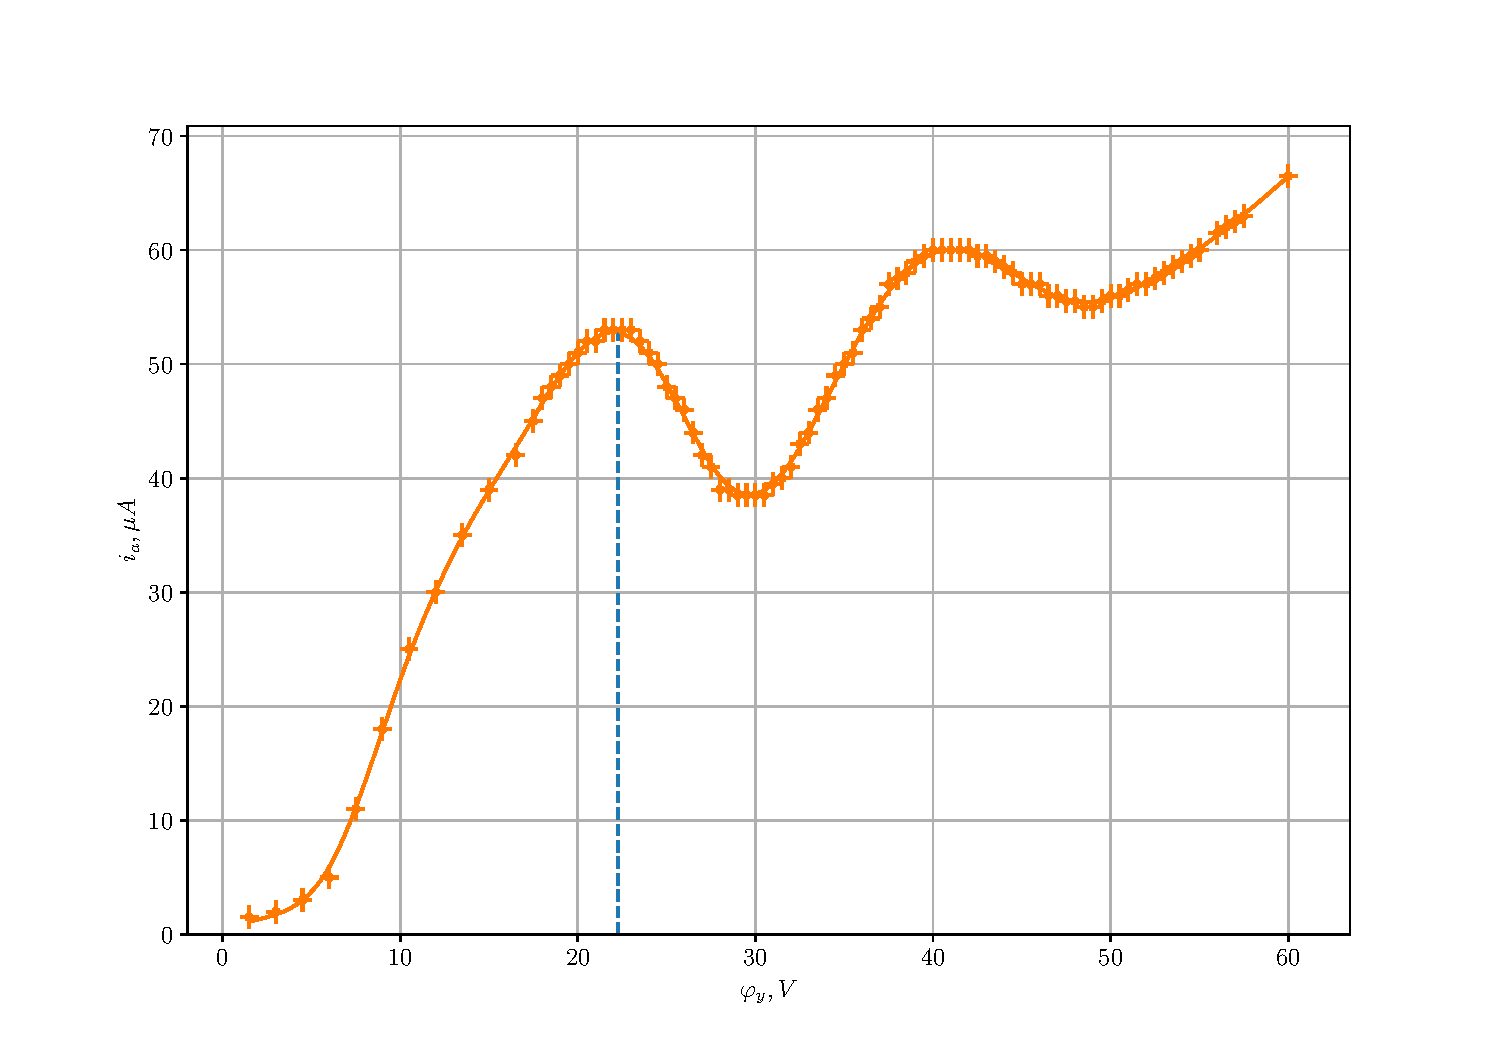
\includegraphics[width=\linewidth]{experiment/Fr-Hz1.pdf}
	\caption{Анодно-сеточная характеристика резонансного потенциала}
	\label{fig1}
\end{figure}
\subsection{Определение ионизационного потенциала}
Сняли анодно-сеточные характеристики для 3 значениях $\phi_\text{з}$. По полученным данным потенциал ионизации составил 28 В. Потенциал ионизации $\phi_\text{и}$определялся как значительное увеличение анодного тока при повышении ускоряющего потенциала. При значениях, близких, но меньше $\phi_\text{и}$ анодный ток может появляться ввиду разброса электронов по скоростям при эмитировании с катода. Электроны, обладающие большей начальной скоростью могут ионизировать атом, при том что большая часть атомов останется не ионизированными. $e(\phi_\text{и}-\phi_1)=5.75$ Эв $<$ $\Delta W_\lambda = e\lambda\frac{d\phi}{dn}\thicksim$ эВ, что является необходимым условием ионизации.
\begin{figure}[h!]
	\vspace{-15pt}
	\centering
	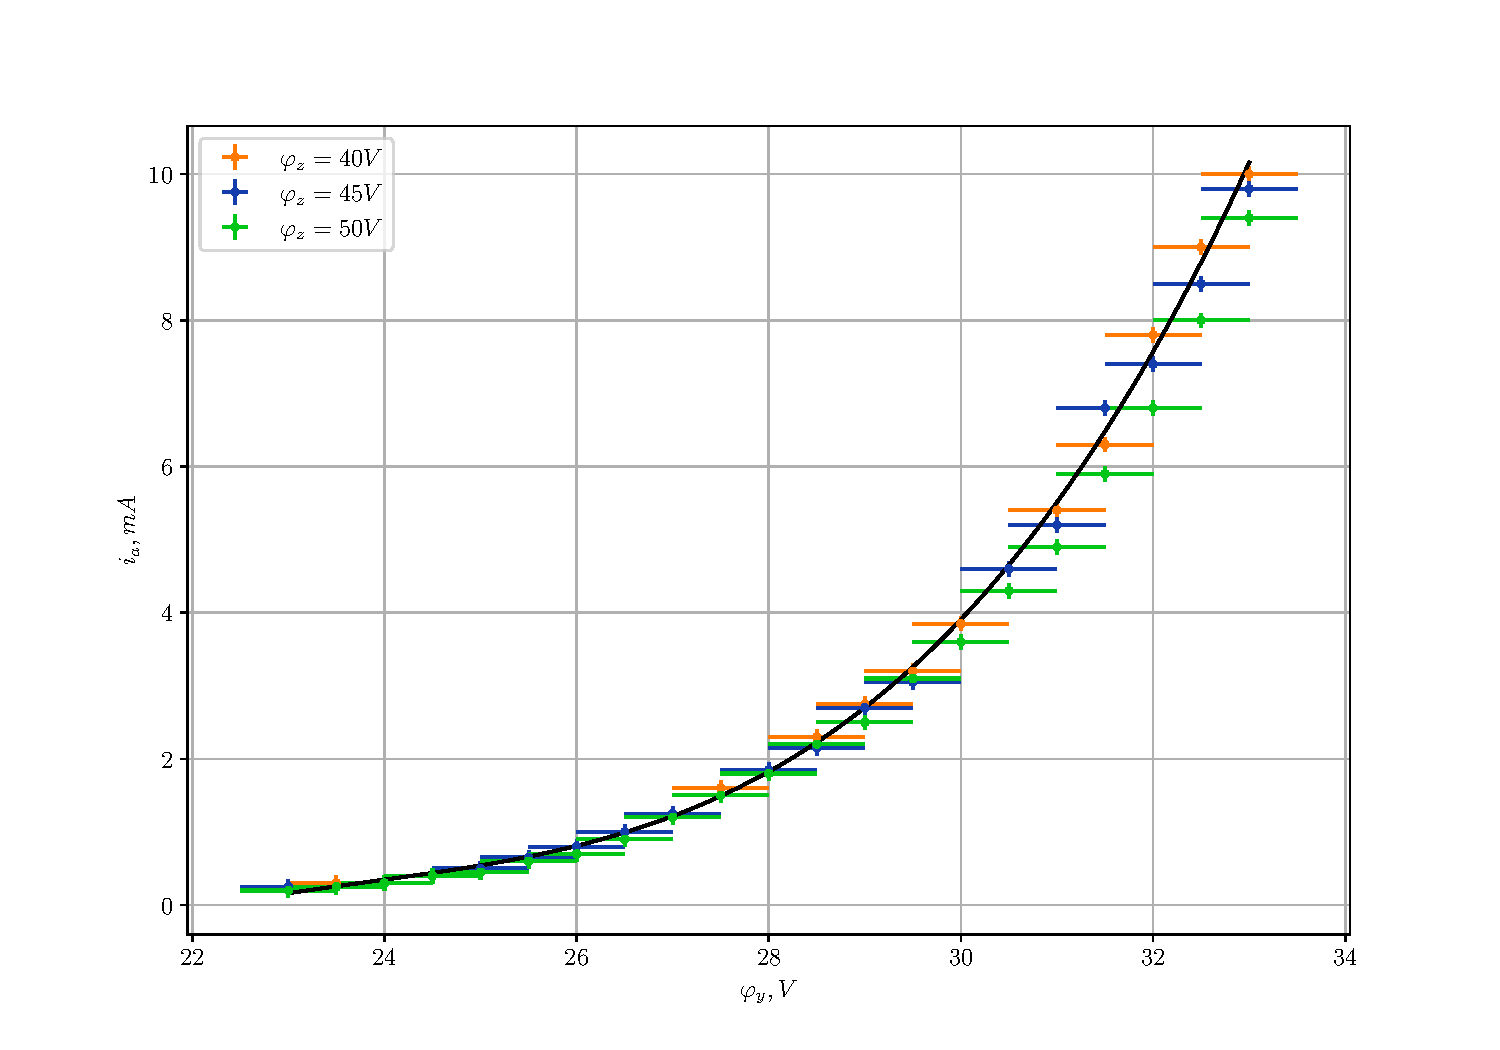
\includegraphics[width=\linewidth]{experiment/Fr-Hz2.pdf}
	\caption{Анодно-сеточная характеристика потенциала ионизации}
	\label{fig:figure1}
\end{figure}

\section{Вывод}
В проведенной работе был экспериментально подтвержден вид сеточной характеристики и ионного тока, которые подтверждают квантовые постулаты Бора. Был определен резонансный и ионизационный потенциалы для гелия.(well done) 

\end{document}